\documentclass[aspectratio=169]{beamer}

\usepackage[utf8]{inputenc}
\usecolortheme{beaver}
\usepackage{caption}
\usepackage{subcaption}
\usepackage{mathtools}
\usepackage{todonotes}
\usepackage{amsmath}
\usepackage{bm}
\usepackage{listings}
\usepackage{ragged2e}
\usepackage{titlecaps}
\usepackage{fancyvrb}
\usepackage[export]{adjustbox}
\usetikzlibrary{arrows}
\usetikzlibrary{shapes}
\def\ci{\perp\!\!\!\!\!\perp}
\newcommand{\cmark}{\ding{51}}
\newcommand{\xmark}{\ding{55}}

\newtheorem{proposition}{Proposition}
\Addlcwords{for a is but and with of in as the etc on to if}

\newcommand{\stackwords}[4]{\begin{tabular}[t]{@{}l@{}l@{}l@{}}#1\\#2\\#3\\#4\end{tabular}}

\setbeamertemplate{section in toc}{\inserttocsectionnumber.~\inserttocsection}
\usetheme{Boadilla}
\makeatletter
\setbeamertemplate{footline}{%
    \leavevmode%
    \hbox{%
        \begin{beamercolorbox}[wd=.3\paperwidth,ht=2.25ex,dp=1ex,center]{author in head/foot}%
            \usebeamerfont{author in head/foot}\insertshortauthor\expandafter\beamer@ifempty\expandafter{\beamer@shortinstitute}{}{~~(\insertshortinstitute)}
        \end{beamercolorbox}%
        \begin{beamercolorbox}[wd=.55\paperwidth,ht=2.25ex,dp=1ex,center]{title in head/foot}%
            \usebeamerfont{title in head/foot}\insertshorttitle
        \end{beamercolorbox}%
        \begin{beamercolorbox}[wd=.15\paperwidth,ht=2.25ex,dp=1ex,right]{date in head/foot}%
            \usebeamerfont{date in head/foot}\insertshortdate{}\hspace*{2em}
            \insertframenumber{} / \inserttotalframenumber\hspace*{2ex} 
        \end{beamercolorbox}}%
        \vskip0pt%
    }
\makeatother

\begin{document}

\title{Testing and Estimation in Causal Models}
\subtitle{Addressing Mixed and Missing Data Challenges}
\author{Ankur Ankan}
\institute[]{Radboud University, The Netherlands}
\date{}

\maketitle

\begin{frame}{Causal Inference}
	\center{Many questions in science are causal.}
	\vspace{1em}
	\only<2>{
	\begin{figure}
		\center
		\begin{subfigure}{0.3 \textwidth}
			\center
			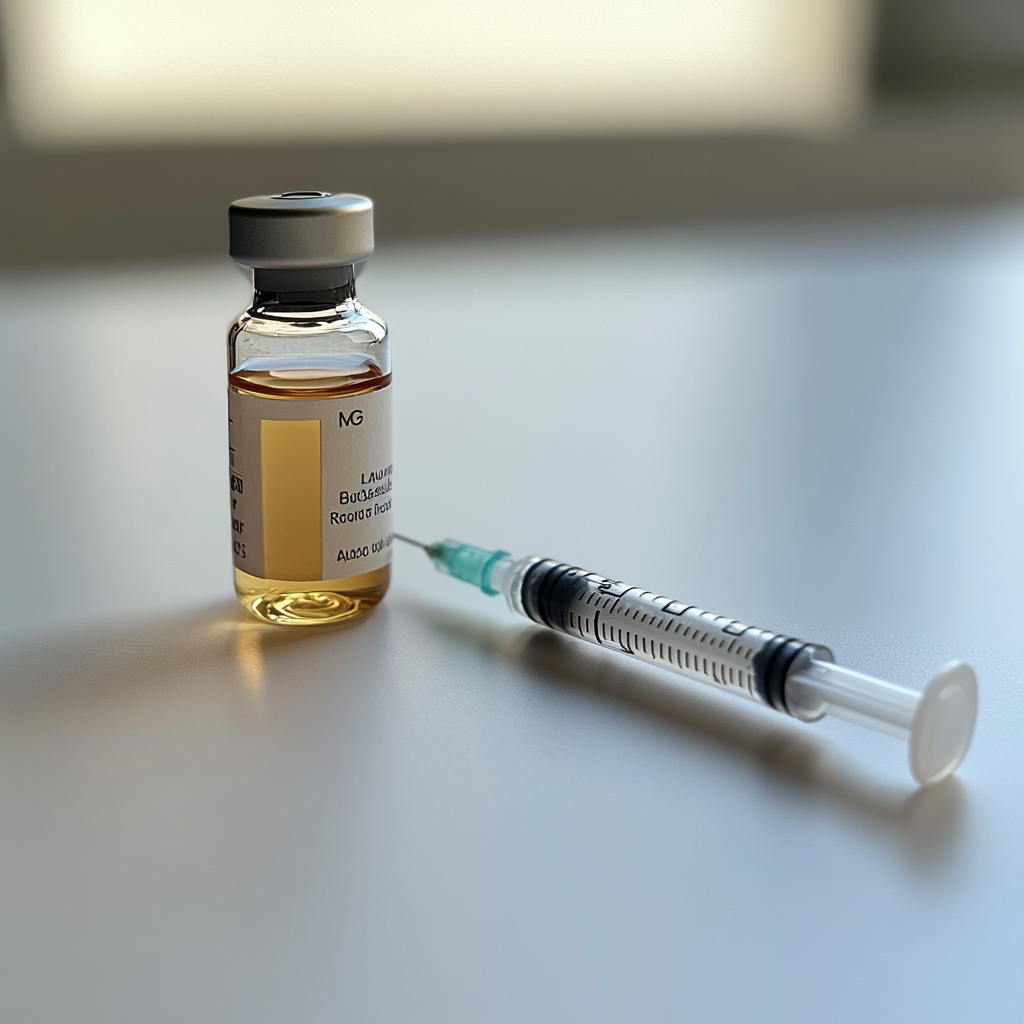
\includegraphics[scale=0.1, valign=m]{imgs/vaccine.png}
		\end{subfigure}
		\qquad\tikz[baseline=-\baselineskip]\draw[ultra thick,->] (-1,0) -- ++ (1,0);\qquad	
		\begin{subfigure}{0.3 \textwidth}
			\center
			
\includegraphics[scale=0.1, valign=m]{imgs/infectious.png}
		\end{subfigure}
	\end{figure}

	\vspace{1em}
	Epidemiology: Does vaccination reduce the spread of infectious disease?
	}
	\only<3>{
	\begin{figure}
		\center
		\begin{subfigure}{0.35 \textwidth}
			\center
			
\includegraphics[scale=0.1, valign=m]{imgs/video_game.png}
		\end{subfigure}
		\qquad\tikz[baseline=-\baselineskip]\draw[ultra thick,->] (0,0) -- ++ (1,0);\qquad	
		\begin{subfigure}{0.35 \textwidth}
			\center
			
\includegraphics[scale=0.1, valign=m]{imgs/fight.png}
		\end{subfigure}
	\end{figure}
	\vspace{1em}
	Social Science: Does exposure to violent video games increase aggressive behavior in children?
	}
	\only<4>{
	\begin{figure}
		\center
		\begin{subfigure}{0.35 \textwidth}
			\center
			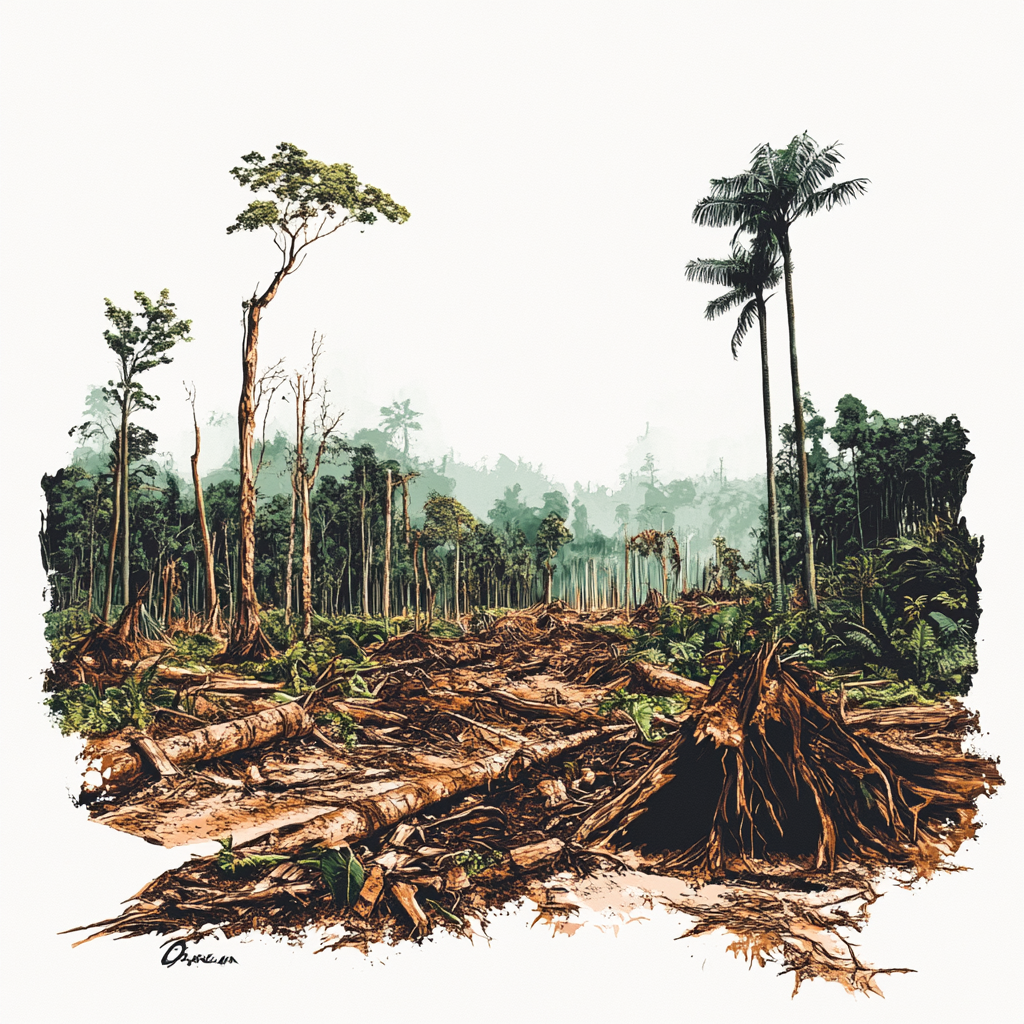
\includegraphics[scale=0.1, valign=m]{imgs/deforestation.png}
		\end{subfigure}
		\qquad\tikz[baseline=-\baselineskip]\draw[ultra thick,->] (0,0) -- ++ (1,0);\qquad	
		\begin{subfigure}{0.35 \textwidth}
			\center
			
\includegraphics[scale=0.1, valign=m]{imgs/climate_change.png}
		\end{subfigure}
	\end{figure}
	\vspace{1em}
	Environmental Science: Does deforestation contribute to climate change?
	}
\end{frame}

\begin{frame}{Causal Inference}
	\begin{tabular}{cccc}
		Understand how an \textbf{intervention} on an & \textbf{exposure} & influences an & \textbf{outcome}. \\
							      & vaccination & & infection spread \\
							      & video games & & aggressive behavior \\
							      & deforestation & & climate change \\
	\end{tabular}
	\vspace{2em}

	\begin{itemize}
		\item \textbf{Understanding Causal Relationships: }
			\begin{itemize}
				\item Is there a causal relationship between the exposure and the outcome.
				\item What kind of relationship? Direct, indirect, common cause, so on.
			\end{itemize}
		\item \textbf{Quantifying Causal Relationships: }
			\begin{itemize}
				\item Measure the magnitude of intervention's impact.
				\item For example, by how much would vaccination reduce spread of infection.
			\end{itemize}
	\end{itemize}
\end{frame}

\begin{frame}{Randomized Controlled Trial}	
	\center{Best way to answer these causal questions is using \textbf{Randomized Controlled Trials}.}
	\todo[inline]{Insert a figure here}
\end{frame}

\begin{frame}{Randomized Controlled Trial}
	\center{However, randomized controlled trials are \textbf{not always feasible.}}
	
	\vspace{2em}

	\begin{itemize}[<+->]
		\item \textbf{Unethical: } To study the effect of smoking on lung cancer, we can not ask non-smokers to start smoking.
		\item \textbf{Difficult to control exposures:} To study the effects of deforestation on climate, we can not create a clones of earth.
		\item \textbf{Cost:} Assessing the effect of education on income would require decades of tracking individuals.
	\end{itemize}

	\vspace{2em}

\only<4>{
\center{Can we answer these questions using data that we already have?}
}
\end{frame}

\begin{frame}{Causal Graphs}
	\center{Yes, but requires understanding the causal mechanism.}
	\vspace{1em}
	\begin{figure}
		\begin{overprint}
			\onslide<1> \center \includegraphics[page=1]{figures.pdf}
			\onslide<2> \center \includegraphics[page=2]{figures.pdf}
			\onslide<3> \center \includegraphics[page=3]{figures.pdf}
			\onslide<4> \center \includegraphics[page=4]{figures.pdf}
		\end{overprint}
	\end{figure}

	\vspace{1em}
\only<4>{
	\begin{itemize}
		\item Understanding causal relationship $ \implies $ Constructing the causal graph.
		\item Quantifying causal relationships $ \implies $ Estimating the edge strengths.
	\end{itemize}
}
\end{frame}

% \begin{frame}{Mixed and Missing Data}
% 	\center{I have focused on improving these methods for mixed and missing data.}
% 
% 	\vspace{2em}
% 
% 	\begin{itemize}
% 		\item \textbf{Mixed Data:}
% 			\begin{enumerate}
% 				\item Numerical:
% 				\item Categorical:
% 				\item Ordinal:
% 			\end{enumerate}
% 
% 		\item \textbf{Missing Data:} Not all variables can be measured. For example climate change.
% 	\end{itemize}
% \end{frame}

\begin{frame}{Constructing Causal Graphs}
\center{How to construct causal graphs?}

\vspace{2em}

\begin{itemize}
	\item Usually constructed manually based on domain knowledge.
	\item Important to test whether our causal graph is correct.
\end{itemize}

\vspace{1em}

\begin{figure}
	\center
	\includegraphics[page=5]{figures.pdf}
\end{figure}
	
\end{frame}

\begin{frame}{Testing Causal Graphs}
	% \begin{figure}
	% 	\includegraphics[page=5]{figures.pdf}
	% \end{figure}
	\begin{itemize}
		\item Selecting the appropriate conditional independence test depends on a
	lot of factors.
	\end{itemize}

	\vspace{1em}
		
	\center{To help researchers to carry out model testing, we wrote a comprehensive guide for selecting appropriate tests for their data.}
\end{frame}

\begin{frame}{Constructing Causal Graphs}
	\begin{figure}
		\center
		\includegraphics[page=6]{figures.pdf}
	\end{figure}

	\begin{itemize}
		\item Both model testing and automatically constructing the graphs require that the statistical tests are accurate.
		\item Incorrect test $ \implies $ Incorrect edge.
		\item Hence, we want these tests to be as accurate as possible.
	\end{itemize}
	
	\center{We proposed a new conditional independence test that can work
	on mixed data and is more accurate than previous methods.}
\end{frame}

\begin{frame}{Causal Effect Estimation}

	\begin{itemize}
		\item If variables can be measured, we have methods to estimate the causal effect between them.
		\item But not always possible to measure variables. For example, we can not directly measure climate change.
		\item Such variables need to measured using other variables. Such as climate change can be measured using variables like:
			\begin{itemize}
				\item Global Average Temperature
				\item Sea Level Rise
				\item Atmospheric CO2 concentration
			\end{itemize}
	\end{itemize}

	\center{We developed a new method to be able to estimate effects between variables that can not be measured.}
\end{frame}

\begin{frame}{Future research}
	\begin{itemize}
		\item We plan to further improve the conditional independence test that we proposed.
		\item We would like to combine the testing and estimation approach to come up with an interpretable metric for mixed data.
	\end{itemize}
\end{frame}

\begin{frame}
	\Huge{Thank you}
\end{frame}

\end{document}
